\subsection{Studies of data from {\asas}}
\protect\label{section:asas}

{\asas} data is available over approximately a decade, although the observations
are taken less frequently than with \ktwo. A plot of the data is shown in Fig.
\ref{fig:asasall}. Again, flaring data obscures several of the observations, but
it was possible to find a number of periods in the data during which little or no flaring took place. In Fig. \ref{fig:asaslcurve} is
shown one such period and the light curve. A periodogram was produced from this,
showing a peak at 2.87 days as shown in Fig. \ref{fig:asaspgram}. Similar
results were obtained from the other periods which did not appear to be affected
by flaring.

\begin{figure}[!htbp]
\begin{center}
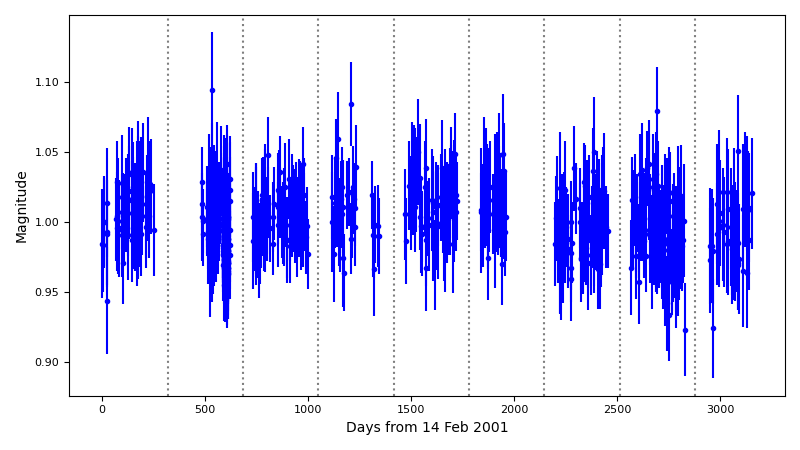
\includegraphics[scale=0.40]{asas/images/asasall.png} \\
\vspace{-.5cm}
\end{center}   
\caption{Data for {\ross} taken from the {\asas} archive selecting only Class A
and B data, converting magnitude and errors to flux values and ignoring data
outside 3 standard deviations from the mean.
The dotted vertical lines show the year divisions. The recommended aperture (2) was used.}\protect\label{fig:asasall}
\end{figure}

\begin{figure}[!htbp]
\begin{center}
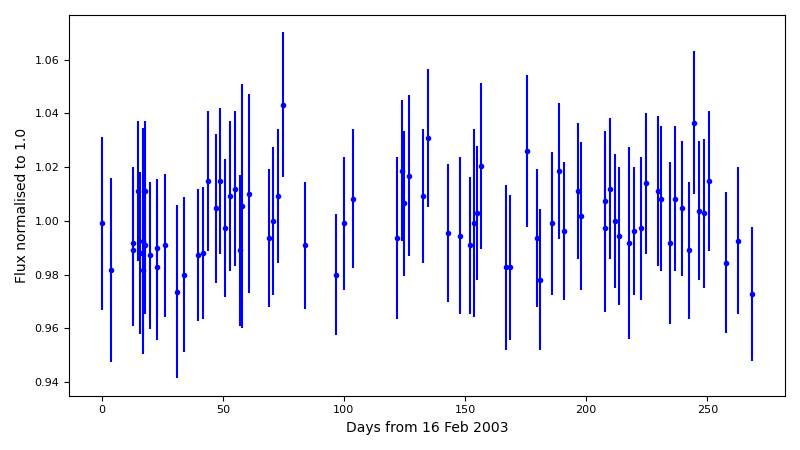
\includegraphics[scale=0.40]{asas/images/asaslcurve.png} \\
\vspace{-.5cm}
\end{center}   
\caption{Subset of Fig. \ref{fig:asasall}, showing {\asas} data for {\ross}
taken from the archive for nearly a year from February 2003, converting
magnitude and errors to flux values and selecting only Class A and B data and
ignoring data outside 3 standard deviations.
This display shows the reported error bar for each observation, the reported magnitude
value being shown as a single point. The
recommended aperture (2) was used.}\protect\label{fig:asaslcurve}
\end{figure}

\begin{figure}[!htbp]
\begin{center}
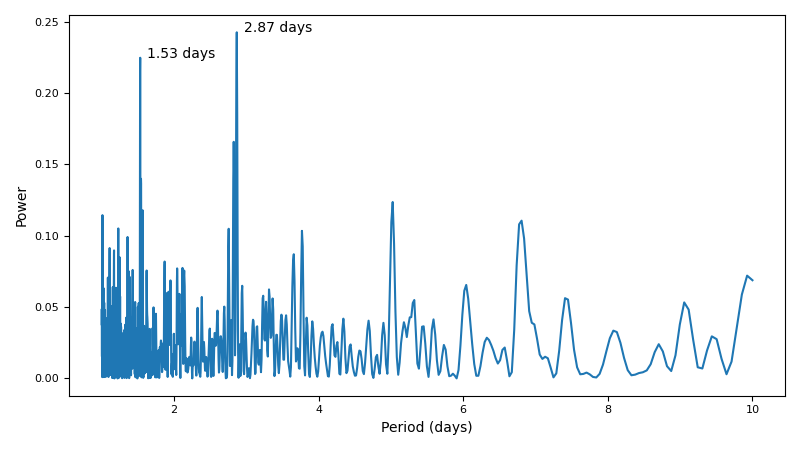
\includegraphics[scale=0.40]{asas/images/asaspgram.png} \\
\vspace{-.5cm}
\end{center}   
\caption{Periodogram taken from the data displayed in Fig.
\ref{fig:asaslcurve}. Again, periods less than 1
day are not considered as the window function (not shown here) reveal numerous
peaks below one day, similar to those shown in Section
\ref{section:k2data}}\protect\label{fig:asaspgram}
\end{figure}

This would again confirm a rotation period of 2.87 days as suggested from the K2
results above in Section \ref{section:k2data}.

